% answers.tex —— 1962 年·全国卷 · 参考答案与详细解析片段
% 由 tools/generate_projects.py 依来源总账自 1962/1962_数学真题_试题.md + 1962/1962_数学真题_解析正文.md + 1962/1962_数学真题_答案要点.md 生成，勿手改（改源 MD 后重跑）


\gkpart{一、小题}

\begin{answer}
\gksolhead{1}{}

\textbf{题目}：

某工厂第三年的产量比第一年的产量增长 $21\%$。问平均每年比上一年增长百分之几？又第一年的产量是第三年的产量的百分之几？（精确到 $1\%$。）

\Needspace{4\baselineskip}
\textbf{解析}

\Needspace{5\baselineskip}
设每年平均增长率为 $x\%$。以第一年的产量为基数，经过两年增长后，第三年的产量满足

\nopagebreak[4]
\[
\left(1+\frac{x}{100}\right)^2=\frac{121}{100}
\]

\Needspace{5\baselineskip}
增长率取正值，所以

\nopagebreak[4]
\[
1+\frac{x}{100}=\frac{11}{10},
\qquad x=10
\]

因此每年平均增长 $10\%$。

\Needspace{5\baselineskip}
第一年产量与第三年产量之比为

\nopagebreak[4]
\[
1\mathbin{:}\frac{121}{100}=\frac{100}{121}\approx0.8264
\]

按题意精确到 $1\%$，第一年产量约为第三年的 $83\%$。

\gkanswer{答案：每年平均增长 $10\%$；第一年产量是第三年的 $83\%$（精确到 $1\%$）。}

\end{answer}
\begin{answer}
\gksolhead{2}{}

\textbf{题目}：

求 $(1-2i)^5$ 的实部。

\Needspace{4\baselineskip}
\textbf{解析}

\Needspace{5\baselineskip}
由二项式展开，实部只来自偶数次项：

\nopagebreak[4]
\[
(1-2i)^5
=1+\binom52(-2i)^2+\binom54(-2i)^4+\text{（纯虚部）}
\]

\Needspace{5\baselineskip}
所以实部为

\nopagebreak[4]
\[
1+10(-2i)^2+5(-2i)^4
=1-40+80=41
\]

\gkanswer{答案：$(1-2i)^5$ 的实部为 $41$。}

\end{answer}
\begin{answer}
\gksolhead{3}{}

\textbf{题目}：

\Needspace{5\baselineskip}
解方程：

\nopagebreak[4]
\[
\log(x-5)+\log(x+3)-2\log2=\log(2x-9)
\]

\Needspace{4\baselineskip}
\textbf{解析}

\Needspace{5\baselineskip}
原方程有意义必须满足

\nopagebreak[4]
\[
x-5>0,
\qquad x+3>0,
\qquad 2x-9>0
\]

\Needspace{5\baselineskip}
因此定义域合并为 $x>5$。在这个定义域内，利用对数的运算性质，原方程可化为

\nopagebreak[4]
\[
\log\frac{(x-5)(x+3)}4=\log(2x-9)
\]

\Needspace{5\baselineskip}
于是

\nopagebreak[4]
\[
(x-5)(x+3)=4(2x-9),
\]
\nopagebreak[4]
\[
x^2-10x+21=0,
\qquad (x-3)(x-7)=0
\]

\Needspace{5\baselineskip}
候选值为 $x=3,7$。由定义域 $x>5$，舍去 $x=3$，故

\nopagebreak[4]
\[
x=7
\]

\gkanswer{答案：$x=7$。}

\end{answer}
\begin{answer}
\gksolhead{4}{}

\textbf{题目}：

\Needspace{5\baselineskip}
求

\nopagebreak[4]
\[
\sin\left(2\arcsin\frac45\right)
\]

的值。

\Needspace{4\baselineskip}
\textbf{解析}

\Needspace{5\baselineskip}
设

\nopagebreak[4]
\[
a=\arcsin\frac45,
\qquad 0<a<\frac\pi2
\]

\Needspace{5\baselineskip}
则

\nopagebreak[4]
\[
\sin a=\frac45,
\qquad \cos a=\sqrt{1-\left(\frac45\right)^2}=\frac35
\]

\Needspace{5\baselineskip}
所以

\nopagebreak[4]
\[
\sin\left(2\arcsin\frac45\right)
=\sin2a
=2\sin a\cos a
=2\cdot\frac45\cdot\frac35
=\frac{24}{25}
\]

\gkanswer{答案：$\dfrac{24}{25}$。}

\end{answer}
\gkpart{二、大题}

\begin{answer}
\gksolhead{5}{}

\textbf{题目}：

求证：

（1）圆内接平行四边形是矩形；

（2）圆外切平行四边形是菱形。

\Needspace{4\baselineskip}
\textbf{解析}

\Needspace{5\baselineskip}
（1）设 $ABCD$ 是圆内接平行四边形。平行四边形的对角相等，所以

\nopagebreak[4]
\[
\angle A=\angle C
\]

\Needspace{5\baselineskip}
圆内接四边形的对角互补，故

\nopagebreak[4]
\[
\angle A+\angle C=180^\circ
\]

\Needspace{5\baselineskip}
从而

\nopagebreak[4]
\[
\angle A=\angle C=90^\circ
\]

所以 $ABCD$ 是矩形。
\nopagebreak[4]
\begin{center}% 1962 年全国卷第 5 题：圆内接平行四边形为矩形。
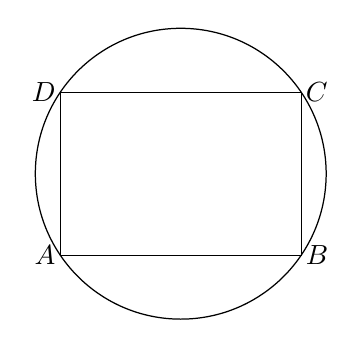
\begin{tikzpicture}[scale=0.9, line width=0.45pt,
  every node/.style={inner sep=1.5pt}]
  \coordinate (A) at (-1.7,-1.15);
  \coordinate (B) at (1.7,-1.15);
  \coordinate (C) at (1.7,1.15);
  \coordinate (D) at (-1.7,1.15);
  \draw (0,0) circle (2.052);
  \draw (A)--(B)--(C)--(D)--cycle;
  \node[anchor=east] at (A) {$A$};
  \node[anchor=west] at (B) {$B$};
  \node[anchor=west] at (C) {$C$};
  \node[anchor=east] at (D) {$D$};
\end{tikzpicture}
\end{center}
\nopagebreak[4]
（2）设平行四边形 $ABCD$ 的四边分别与圆相切，切点依次为 $E,F,G,H$。
\nopagebreak[4]
\begin{center}% 1962 年全国卷第 5 题：圆外切平行四边形为菱形。
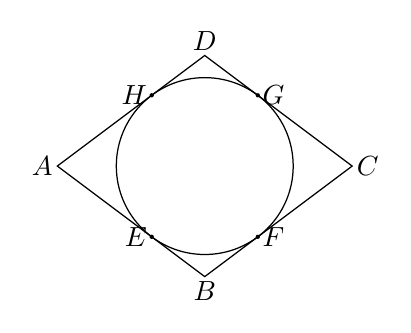
\begin{tikzpicture}[scale=0.78, line width=0.45pt,
  every node/.style={inner sep=1.5pt}]
  \coordinate (A) at (-2.4,0);
  \coordinate (B) at (0,-1.8);
  \coordinate (C) at (2.4,0);
  \coordinate (D) at (0,1.8);
  \coordinate (E) at (-0.864,-1.152);
  \coordinate (F) at (0.864,-1.152);
  \coordinate (G) at (0.864,1.152);
  \coordinate (H) at (-0.864,1.152);
  \draw (0,0) circle (1.44);
  \draw (A)--(B)--(C)--(D)--cycle;
  \fill (E) circle (0.035) (F) circle (0.035) (G) circle (0.035) (H) circle (0.035);
  \node[anchor=east] at (A) {$A$};
  \node[anchor=north] at (B) {$B$};
  \node[anchor=west] at (C) {$C$};
  \node[anchor=south] at (D) {$D$};
  \node[anchor=east] at (E) {$E$};
  \node[anchor=west] at (F) {$F$};
  \node[anchor=west] at (G) {$G$};
  \node[anchor=east] at (H) {$H$};
\end{tikzpicture}
\end{center}
\nopagebreak[4]
\Needspace{5\baselineskip}
由同一点向圆所作的两条切线段相等，得

\nopagebreak[4]
\[
AE=AH,\qquad BE=BF,\qquad CG=CF,\qquad DG=DH
\]

\Needspace{5\baselineskip}
四式相加，得到

\nopagebreak[4]
\[
AB+CD=AD+BC
\]

\Needspace{5\baselineskip}
又因为 $ABCD$ 是平行四边形，

\nopagebreak[4]
\[
AB=CD,\qquad AD=BC
\]

代入上式可得 $AB=BC$。平行四边形有一组邻边相等，所以 $ABCD$ 是菱形。

\gkanswer{答案：圆内接平行四边形为矩形；圆外切平行四边形为菱形。}

\end{answer}
\begin{answer}
\gksolhead{6}{}

\textbf{题目}：

\Needspace{5\baselineskip}
解方程组：

\nopagebreak[4]
\[
\begin{cases}
y^2-4x-2y+1=0,\\
y=x+a
\end{cases}
\]

并讨论：$a$ 取哪些实数值时，这个方程组

（1）有不同的两组实数解；

（2）有相同的两组实数解；

（3）没有实数解。

\Needspace{4\baselineskip}
\textbf{解析}

\Needspace{5\baselineskip}
由第二个方程得

\nopagebreak[4]
\[
x=y-a
\]

\Needspace{5\baselineskip}
代入第一个方程，得

\nopagebreak[4]
\[
y^2-4(y-a)-2y+1=0
\]
\Needspace{5\baselineskip}
即

\nopagebreak[4]
\[
y^2-6y+4a+1=0
\]

\Needspace{5\baselineskip}
解得

\nopagebreak[4]
\[
y=3\pm\sqrt{9-(4a+1)}
=3\pm2\sqrt{2-a}
\]

\Needspace{5\baselineskip}
再由 $x=y-a$，得到两组形式解

\nopagebreak[4]
\[
\begin{cases}
x_1=3-a+2\sqrt{2-a},\\
y_1=3+2\sqrt{2-a},
\end{cases}
\qquad
\begin{cases}
x_2=3-a-2\sqrt{2-a},\\
y_2=3-2\sqrt{2-a}
\end{cases}
\]

要有实数解，必须 $2-a\ge0$。

\begin{itemize}
\item 当 $a<2$ 时，根号内为正，两组解不同；
\item 当 $a=2$ 时，根号项为零，两组解相同，均为 $(x,y)=(1,3)$；
\item 当 $a>2$ 时，根号内为负，没有实数解。
\end{itemize}

\gkanswer{答案：$(x,y)=\left(3-a\pm2\sqrt{2-a},\,3\pm2\sqrt{2-a}\right)$（两组解取同号），其中 $2-a\geqslant0$。}

\end{answer}
\begin{answer}
\gksolhead{7}{}

\textbf{题目}：

如图，$ABCD$ 和 $A'B'C'D'$ 都是正方形，而 $A'$、$B'$、$C'$、$D'$ 顺次分别把 $AB$、$BC$、$CD$、$DA$ 分成 $m:n$，并设 $AB=1$。
\nopagebreak[4]
\begin{center}% 1962 年全国卷第 7 题：正方形边上按 m:n 分点形成内接正方形。
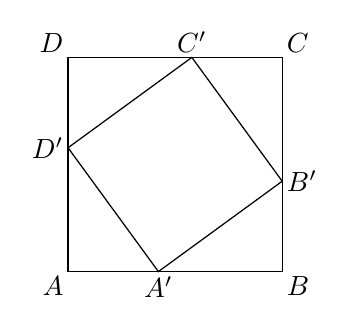
\begin{tikzpicture}[scale=0.85, line width=0.45pt,
  every node/.style={inner sep=1.5pt}]
  \coordinate (A) at (0,0);
  \coordinate (B) at (3.2,0);
  \coordinate (C) at (3.2,3.2);
  \coordinate (D) at (0,3.2);
  \coordinate (Ap) at (1.35,0);
  \coordinate (Bp) at (3.2,1.35);
  \coordinate (Cp) at (1.85,3.2);
  \coordinate (Dp) at (0,1.85);
  \draw (A)--(B)--(C)--(D)--cycle;
  \draw (Ap)--(Bp)--(Cp)--(Dp)--cycle;
  \node[anchor=north east] at (A) {$A$};
  \node[anchor=north west] at (B) {$B$};
  \node[anchor=south west] at (C) {$C$};
  \node[anchor=south east] at (D) {$D$};
  \node[anchor=north] at (Ap) {$A'$};
  \node[anchor=west] at (Bp) {$B'$};
  \node[anchor=south] at (Cp) {$C'$};
  \node[anchor=east] at (Dp) {$D'$};
\end{tikzpicture}
\end{center}
\nopagebreak[4]
（1）求正方形 $A'B'C'D'$ 的面积；

（2）证明：正方形 $A'B'C'D'$ 的面积不小于 $\dfrac12$。

\Needspace{4\baselineskip}
\textbf{解析}

\Needspace{5\baselineskip}
因为 $AB=1$ 且 $AA':A'B=m:n$，所以

\nopagebreak[4]
\[
AA'=\frac{m}{m+n},
\qquad A'B=\frac{n}{m+n}
\]

\Needspace{5\baselineskip}
在直角三角形 $A'BB'$ 中，$BB'=AA'$，故

\nopagebreak[4]
\[
A'B'
=\sqrt{A'B^2+BB'^2}
=\sqrt{A'B^2+AA'^2}
=\sqrt{\frac{m^2+n^2}{(m+n)^2}}
\]

\Needspace{5\baselineskip}
由于 $A'B'C'D'$ 是正方形，其面积为

\nopagebreak[4]
\[
S= A'B'^2=\frac{m^2+n^2}{(m+n)^2}
\]

\Needspace{5\baselineskip}
再证下界：

\nopagebreak[4]
\[
\frac{m^2+n^2}{(m+n)^2}-\frac12
=\frac{2(m^2+n^2)-(m+n)^2}{2(m+n)^2}
=\frac{(m-n)^2}{2(m+n)^2}\ge0
\]

\Needspace{5\baselineskip}
因此

\nopagebreak[4]
\[
S\ge\frac12
\]

\gkanswer{答案：正方形 $A'B'C'D'$ 的面积为 $\dfrac{m^2+n^2}{(m+n)^2}$，且不小于 $\dfrac12$。}

\end{answer}
\begin{answer}
\gksolhead{8}{}

\textbf{题目}：

\Needspace{5\baselineskip}
$D$ 是 $\triangle ABC$ 内的一点，已知

\nopagebreak[4]
\[
AB=AC=1,\qquad \angle CAB=63^\circ,
\qquad \angle DAB=33^\circ,\qquad \angle DBA=27^\circ,
\]

求 $CD$。（$\sin27^\circ=0.4540$。最后结果计算到小数点后两位。）

\Needspace{4\baselineskip}
\textbf{解析}
\nopagebreak[4]
\begin{center}% 1962 年全国卷第 8 题：等腰三角形中的内点 D。
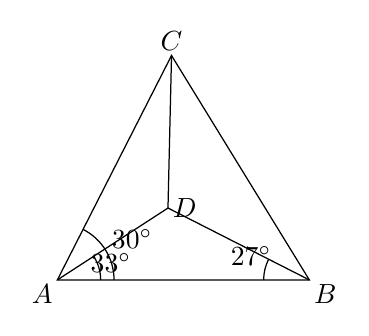
\begin{tikzpicture}[scale=1.0, line width=0.45pt,
  every node/.style={inner sep=1.5pt}]
  \coordinate (A) at (0,0);
  \coordinate (B) at (3.2,0);
  \coordinate (C) at (1.45,2.85);
  \coordinate (D) at (1.405,0.913);
  \draw (A)--(B)--(C)--cycle;
  \draw (A)--(D)--(B);
  \draw (C)--(D);
  \draw (0.55,0) arc (0:33:0.55);
  \draw (0.72,0) arc (0:63:0.72);
  \draw (2.62,0) arc (180:153:0.58);
  \node[anchor=north east] at (A) {$A$};
  \node[anchor=north west] at (B) {$B$};
  \node[anchor=south] at (C) {$C$};
  \node[anchor=west] at (D) {$D$};
  \node at (0.68,0.22) {$33^\circ$};
  \node at (0.95,0.52) {$30^\circ$};
  \node at (2.46,0.3) {$27^\circ$};
\end{tikzpicture}
\end{center}
\nopagebreak[4]
\Needspace{5\baselineskip}
在 $\triangle ABD$ 中，

\nopagebreak[4]
\[
\angle BDA=180^\circ-33^\circ-27^\circ=120^\circ
\]

\Needspace{5\baselineskip}
由正弦定理，

\nopagebreak[4]
\[
\frac{AD}{\sin27^\circ}=\frac{AB}{\sin120^\circ}
=\frac1{\sin120^\circ}
\]

\Needspace{5\baselineskip}
所以

\nopagebreak[4]
\[
AD=\frac2{\sqrt3}\sin27^\circ
\]

\Needspace{5\baselineskip}
又

\nopagebreak[4]
\[
\angle DAC=63^\circ-33^\circ=30^\circ
\]

\Needspace{5\baselineskip}
在 $\triangle ADC$ 中使用余弦定理：

\nopagebreak[4]
\[
CD^2=AC^2+AD^2-2AC\cdot AD\cos30^\circ
\]

\nopagebreak[4]
\[
CD^2=1+\frac43\sin^227^\circ-2\sin27^\circ
\]

\Needspace{5\baselineskip}
代入题给 $\sin27^\circ=0.4540$，得

\nopagebreak[4]
\[
CD^2\approx1+\frac43(0.4540)^2-2(0.4540)
\approx0.3668
\]

\Needspace{5\baselineskip}
因此

\nopagebreak[4]
\[
CD\approx0.6057
\]

按通常四舍五入到小数点后两位为 $0.61$。原卷答案页末行印作 $0.60$，与上述平方根的四舍五入结果不一致，本库保留该差异供核查。

\gkanswer{答案：原卷答案页末行印作 $CD=0.60$；按题面给定 $\sin27^\circ=0.4540$ 直接计算，$CD^2\approx0.3668$，按通常四舍五入到小数点后两位应为 $CD\approx0.61$。}

\end{answer}
\begin{answer}
\gksolhead{9}{}

\textbf{题目}：

\Needspace{5\baselineskip}
由正方体 $ABCD-A_1B_1C_1D_1$ 的顶点 $A$ 作这个正方体的对角线 $A_1C$ 的垂线，垂足为 $E$。证明：

\nopagebreak[4]
\[
A_1E:EC=1:2
\]

（要求画图。）

\Needspace{4\baselineskip}
\textbf{解析}
\nopagebreak[4]
\begin{center}% 1962 年全国卷第 9 题：正方体对角线 A_1C 与垂足 E。
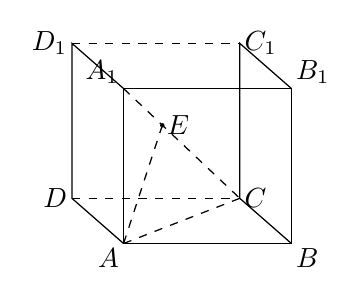
\begin{tikzpicture}[scale=0.82, line width=0.45pt,
  every node/.style={inner sep=1.5pt}]
  \coordinate (A) at (0,0);
  \coordinate (B) at (2.6,0);
  \coordinate (B1) at (2.6,2.4);
  \coordinate (A1) at (0,2.4);
  \coordinate (D) at (-0.8,0.7);
  \coordinate (C) at (1.8,0.7);
  \coordinate (C1) at (1.8,3.1);
  \coordinate (D1) at (-0.8,3.1);
  \coordinate (E) at (0.6,1.83);
  \draw (A)--(B)--(B1)--(A1)--cycle;
  \draw (A)--(D)--(D1)--(A1);
  \draw (B)--(C)--(C1)--(B1);
  \draw[dashed] (D)--(C) (D1)--(C1);
  \draw[dashed] (A1)--(C) (A)--(C) (A)--(E);
  \fill (E) circle (0.035);
  \node[anchor=north east] at (A) {$A$};
  \node[anchor=north west] at (B) {$B$};
  \node[anchor=west] at (C) {$C$};
  \node[anchor=east] at (D) {$D$};
  \node[anchor=south east] at (A1) {$A_1$};
  \node[anchor=south west] at (B1) {$B_1$};
  \node[anchor=west] at (C1) {$C_1$};
  \node[anchor=east] at (D1) {$D_1$};
  \node[anchor=west] at (E) {$E$};
\end{tikzpicture}
\end{center}
\nopagebreak[4]
\Needspace{5\baselineskip}
作对角线 $AC$。因为 $AA_1$ 垂直于正方体底面，且 $AC$ 在底面内，所以

\nopagebreak[4]
\[
AA_1\perp AC
\]

\Needspace{5\baselineskip}
故 $\triangle A_1AC$ 是直角三角形。设正方体棱长为 $1$，则

\nopagebreak[4]
\[
A_1A=1,
\qquad AC=\sqrt2,
\qquad A_1C=\sqrt3
\]

\Needspace{5\baselineskip}
由 $AE\perp A_1C$，利用直角三角形斜边上的高的射影定理，得

\nopagebreak[4]
\[
A_1A^2=A_1E\cdot A_1C,
\qquad 1=A_1E\cdot A_1C
\]

\Needspace{5\baselineskip}
同理，

\nopagebreak[4]
\[
AC^2=EC\cdot A_1C,
\qquad 2=EC\cdot A_1C
\]

\Needspace{5\baselineskip}
因此

\nopagebreak[4]
\[
A_1E:EC=1:2
\]

\gkanswer{答案：$A_1E:EC=1:2$。}

\end{answer}
\begin{answer}
\gksolhead{10}{}

\textbf{题目}：

求证：两两相交而不通过同一点的四条直线必在同一平面内。

\Needspace{4\baselineskip}
\textbf{解析}

在四条直线中任取两条，记为 $a,b$，设交点为 $P$。由四条直线不通过同一点，另外两条直线中至少有一条不通过 $P$，记这条直线为 $c$。

因为直线两两相交，$c$ 分别与 $a,b$ 相交；且 $c$ 不通过 $P$，所以这两个交点是不同的。直线 $a,b$ 决定一个平面，而平面内过这两个不同点的直线唯一，因此 $c$ 在该平面内。

最后，第四条直线 $d$ 分别与 $a,b,c$ 相交。它至少有两个不同的交点落在上述平面内：若 $d$ 通过 $P$，它与 $c$ 的交点不可能也是 $P$，因为 $c$ 不通过 $P$；若 $d$ 不通过 $P$，则它与 $a,b$ 的交点已是两个不同点。于是 $d$ 也在这个平面内。

所以四条直线必在同一平面内。

\gkanswer{答案：两两相交且不共点的四条直线共面。}

\end{answer}